

\chapter{Nb-Substrate Optimization}

    Optimization on Nb substrates before moving to Cu substrates allows a simpler understanding of how the Nb$_3$Sn film is formed. In general, you only have to supply Sn to the Nb substrate, and the Nb$_3$Sn reaction can take place. However, one must optmize the Sn supply so the Nb can have sufficient Sn supply throughout the reaction. We deposited $\sim5$\unit{\um} CuSn film on the polished Nb substrate as the Sn source. 

    \begin{figure}
        \centering
        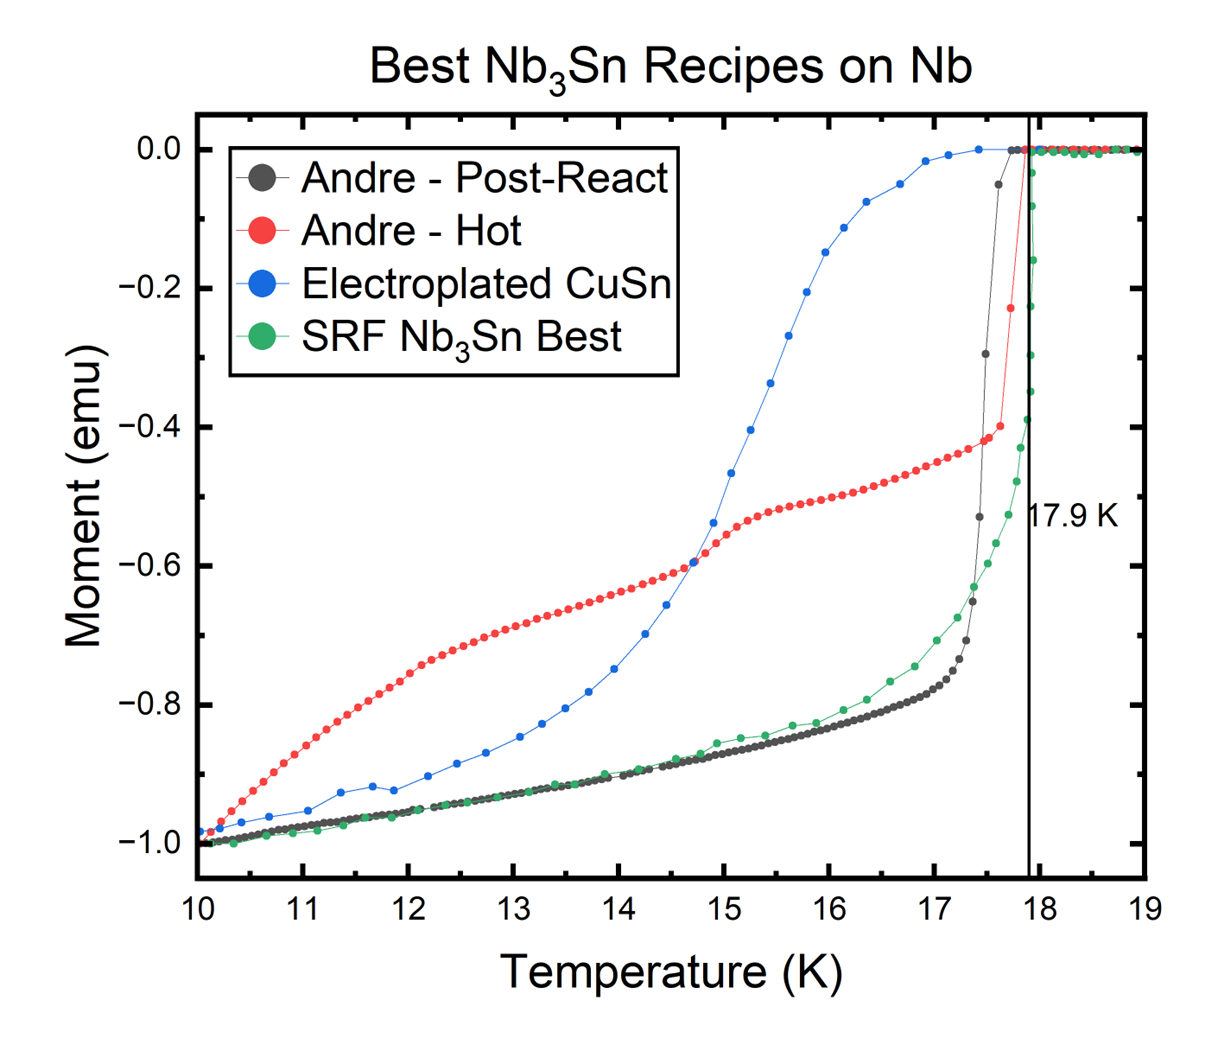
\includegraphics[width=.5\textwidth]{images/Nb/Nb3SnonNbBest.png}
        \caption[$T_c$ curves for best samples on Nb substrate including other groups.]{Critical temperature curves comparing our best post-reacted and hot-bronze sample made on a Nb substrate, to the best Nb$_3$Sn film made with Sn vapor, and an electrochemically processed bronze route Nb$_3$Sn film.}
        \label{fig:Nb3SnonNbBest}
    \end{figure}        
    

        Our goal in this experiment was to understand what Sn concentration is optimal in the Cu-Sn film when reacting with Nb to make Nb$_3$Sn given a reaction time and temperature. This experiment used critical temperature measurements and microstructure analysis to probe the quality of the Nb$_3$Sn films on Nb. The $T_c$ can be near maximum since the CTE mismatch between Nb$_3$Sn and Nb is the smallest of all materials, so the strain is minimal in the film. Therefore, the main contribution to a depression in $T_c$ is sub 25\% at. Sn in the Nb$_3$Sn. 
        
        The first experiment thermally evaporated 3 \si{\um} of different Sn concentrations of Cu-Sn film wt\% Sn: Cu5Sn, Cu13Sn, Cu19Sn, Cu34Sn, and Cu38Sn with different heat-treatment temperatures 650 °C, 700 °C,  750 °C and times 12 hr and 24 hr. These samples were heat-treated in a vacuum furnace pumped down to $10^{-7}$ Torr and back-filled with high-purity argon to mitigate oxygen and nitrogen impurity diffusion into the film during heating.

        %show figure. Where is the Sn going? Vapor pressure.DISCUSSION)
 
        \begin{figure}
            \centering
            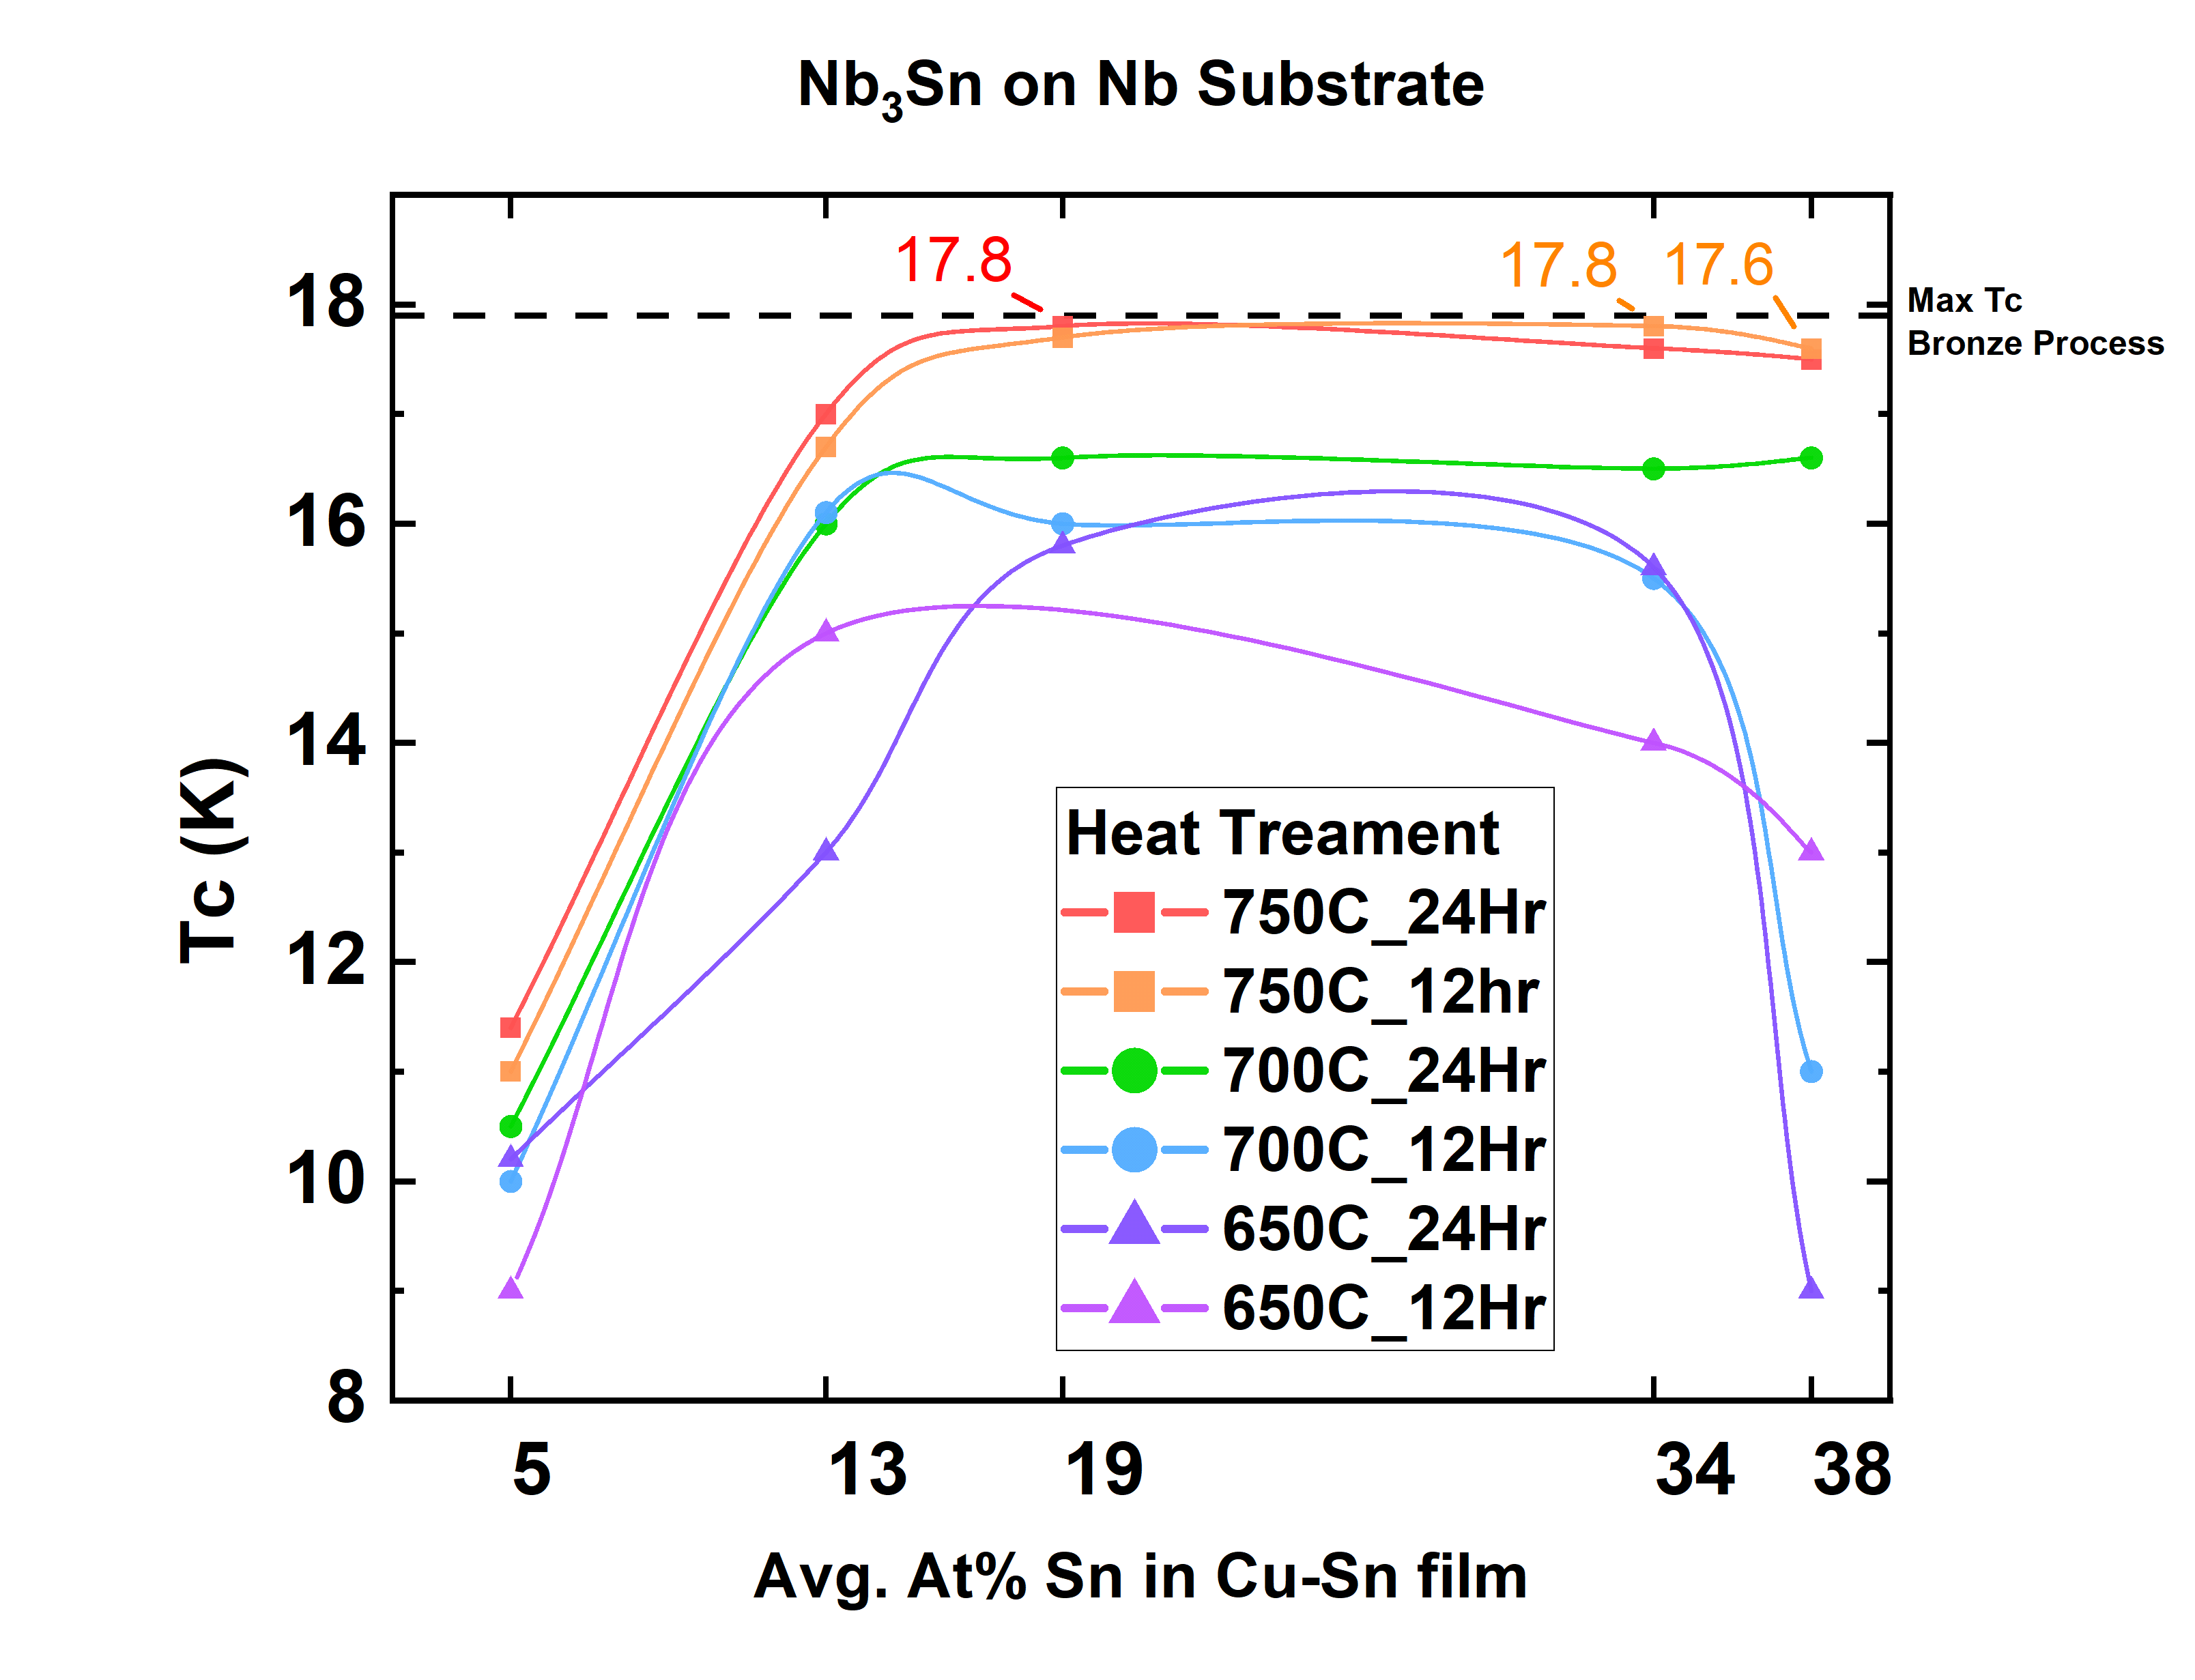
\includegraphics[width=.7\textwidth]{images/Nb/NbSubUpdated.png}
            \caption[$T_c$ onset for recipes varying Cu-Sn film and reaction on Nb substrates.]{$T_c$ curves for 650°C, 700°C and 750°C with 12Hr and 24Hr heat treatments. Sn composition in the Cu-Sn film was varied from 5 to 38 At\% Sn by varying the Sn composition in the Cu-Sn target.} %Sn percentage in the film??
            \label{fig:NbSubUpdated}
        \end{figure}
         
        \begin{figure}
            \centering
            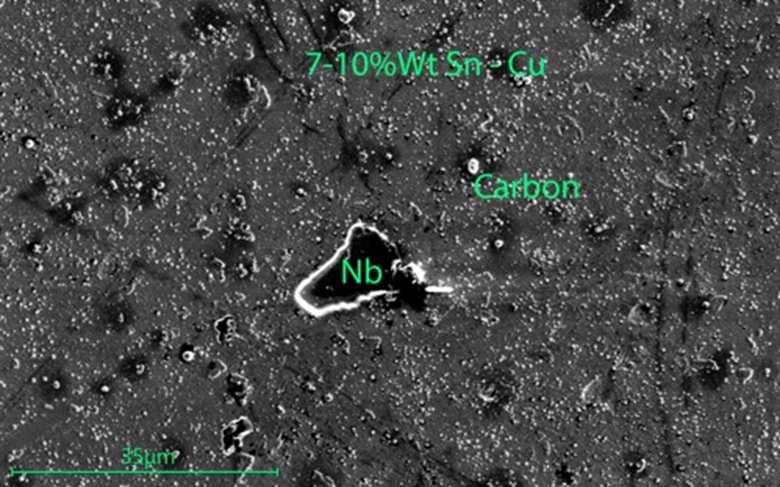
\includegraphics[width=.327\textwidth]{images/Nb/5CuSn.png}
            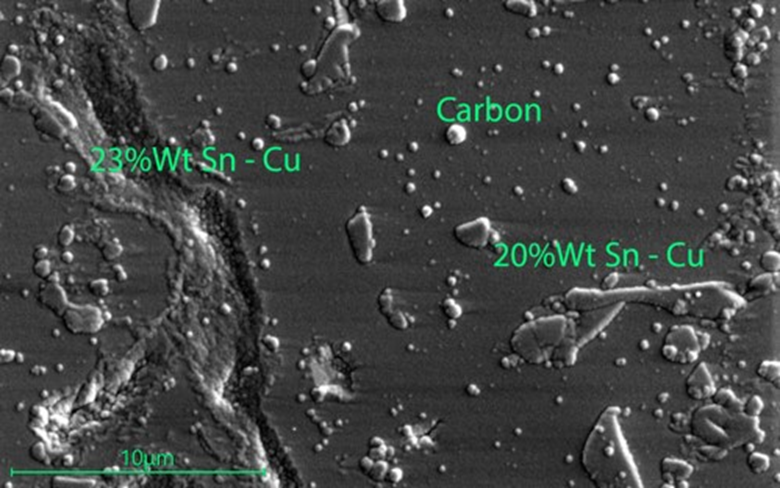
\includegraphics[width=.327\textwidth]{images/Nb/13CuSn.png}
            \\[\smallskipamount]

            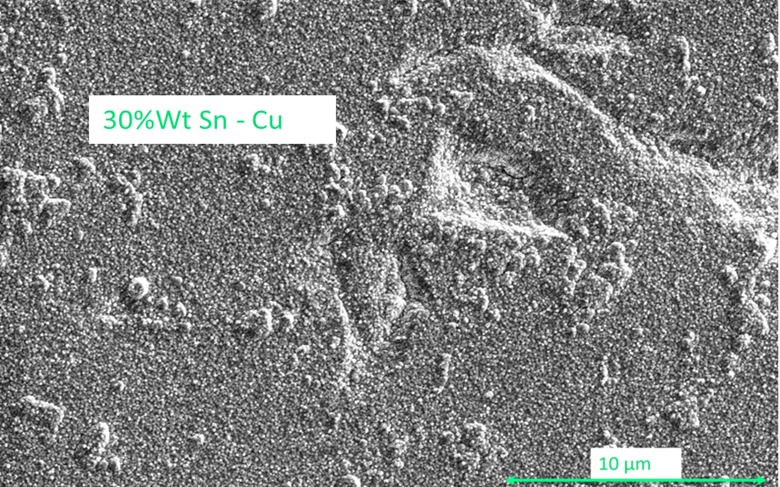
\includegraphics[width=.327\textwidth]{images/Nb/24CuSn.png}\hfill
            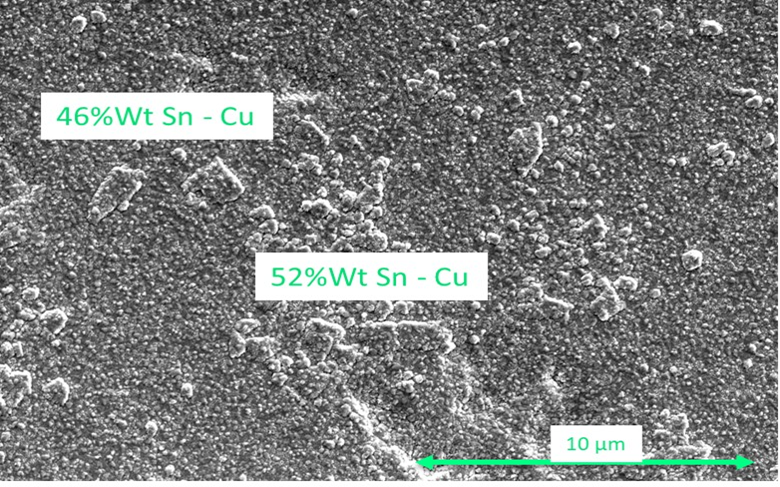
\includegraphics[width=.327\textwidth]{images/Nb/33CuSn.png}\hfill
            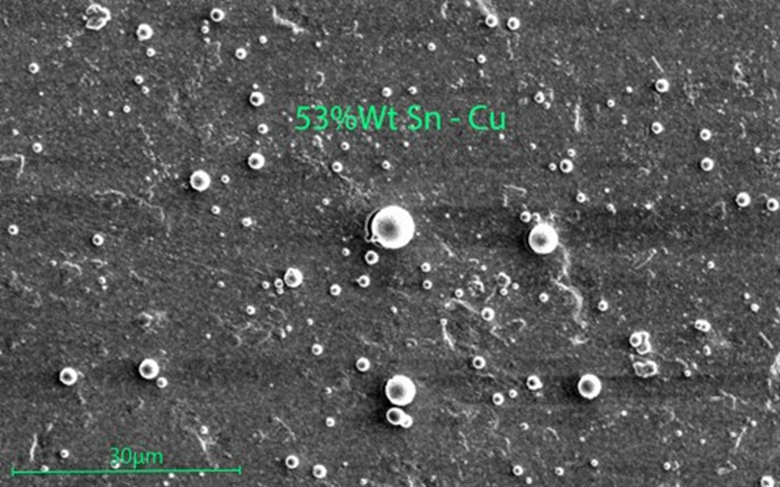
\includegraphics[width=.327\textwidth]{images/Nb/40CuSn.png}
            \caption{2\si{\um} Cu-Sn films made from thermally evaporated targets with compositions of (13,13,24,33,40) wt\% Sn on Nb substrates. 13\% film was made with a different boat, which resulted in a lower Sn film.}
            \label{fig:CuSnOnNb}
        \end{figure}

        The highest $T_c$, 17.8 K, was measured in samples with the highest heat treatment temperature at 750 °C as shown in the legend in Figure \ref{fig:NbSubUpdated}. There was very little difference between the $T_c$ of the 12 Hr and 24 Hr heat treatment as shown in Figure \ref{fig:NbSubUpdated}, though the layer was thicker for the 24 Hr heat treated samples. This increase in $T_c$ aligns with literature \cite{Xu:2017wsa} and follows the general rule that high Sn activity makes good quality Nb$_3$Sn. High Sn diffusion allows for substitution into the Nb lattice at a high rate, allowing Nb$_3$Sn to form in equilibrium with near 25\% perfect stoichiometry. The higher the temperature, the higher the diffusion rate of Sn into the Nb sites. The optimal amount of Sn in the Cu-Sn concentration was 19-34\% at. Sn as seen in Figure \ref{fig:NbSubUpdated}. If there is too little Sn in the Cu-Sn film, there will not be enough Sn volume to substitute into the Nb matrix. The resulting Nb$_3$Sn will have low Sn. If the Cu-Sn film has too high Sn content, around the epsilon single phase at 38\% Cu-Sn, an eta phase can form, which decomposes to less favorable Nb-Sn compounds such as Nb$_6$Sn$_5$ and NbSn$_2$. 
        These will decompose at high temperatures due to high Sn activity, but at lower temperatures, lead to unfavorable microstructure and compositions, giving poor quality Nb$_3$Sn. This explains why the low-temperature curves in \ref{fig:NbSubUpdated} for the 38\% Cu-Sn film have low $T_c$, but the high-temperature films have near max $T_c$. 

        \begin{figure}
            \centering
            \begin{subfigure}{0.49\textwidth}
            \centering
            
\includegraphics[width = \textwidth]{40Nb.png}
            \caption{}
            \label{fig:40Nb}
            \end{subfigure}
            \begin{subfigure}{0.49\textwidth}
            \centering
            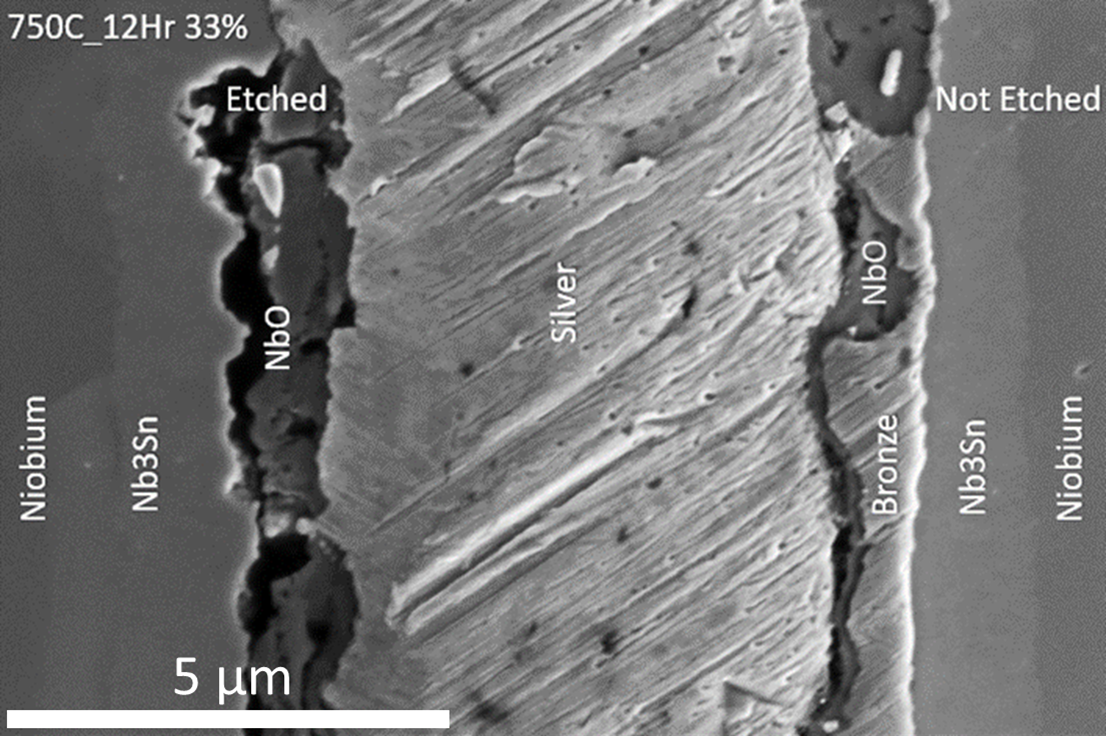
\includegraphics[width = \textwidth]{images/Nb/33NbCut.png}
            \caption{}
            \label{fig:33Nb}
            \end{subfigure}
            \caption[Cross-section showing etched vs not-etched Nb$_3$Sn sample on Nb.]{Comparison of SEM cross-sectional microstructure of a Nb$_3$Sn film that has been etched and left not etched. Both of these cross-sections show an Nb$_3$Sn film that was reacted at 750C for 12Hr with a 2 \si{\um} CuSn layer on top of an Nb substrate. The left image a) shows a film with a 40\% wt Sn Cu-Sn layer, while image b) used a 33\% wt Sn Cu-Sn layer. The noticeable difference is in the twice larger film thickness of the Nb$_3$Sn layer in a) the 40\% Cu-Sn film case compared to the 33\% film with the same heat-treatment.}
            \label{fig:combined}
        \end{figure} 

        A hot bronze sample was made with a Nb substrate to take advantage of the low CTE mismatch between the Nb substrate and Nb$_3$Sn film and use the high Sn activity of the bronze route. A similar structure to the above experiment was built, a Cu-Sn film on a Nb substrate, and then a subsequent Nb layer was sputtered on top of this bilayer at 700 C. This leads to one hot bronze Nb$_3$Sn film above the Cu-Sn film and a second Nb$_3$Sn film below the Cu-Sn film created from solid state diffusion of Sn into the Nb substrate. A cross-section of this film is shown in Figure \ref{fig:NbHot} where one can see the two Nb$_3$Sn films above and below the Cu-Sn film.
        
        \begin{figure}
            \centering
            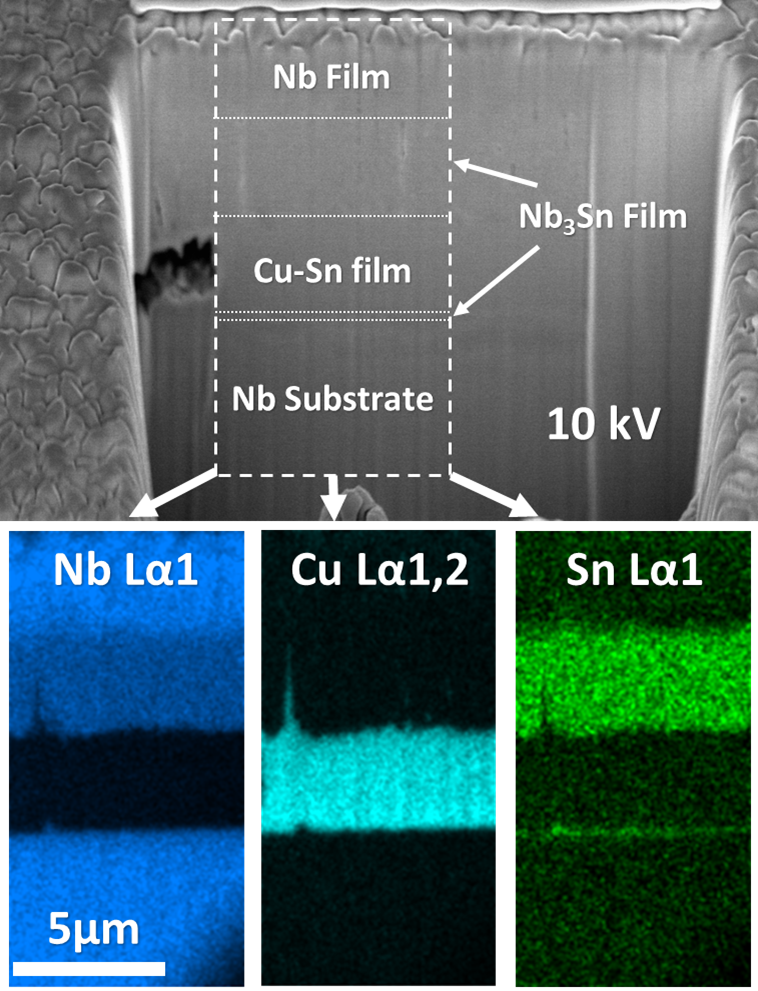
\includegraphics[width=.5\textwidth]{images/Nb/NbHot.png}
            \caption[Cross-section of hot-bronze film on a Nb substrate.]{FIB Cross-section SEM/EDS of two Nb$_3$Sn films on one Nb substrate, one below and one above the Cu-Sn film. One was made using the hot bronze technique, and the other using solid-state diffusion. The full critical temperature curve of this sample is plotted in red curve in Fig. \ref{fig:Nb3SnonNbBest} and is labeled as the 3 $\mu$m film.}
            %(EDS linescan shows 20\% At Sn with 5\% Cu, too large of Cu, would need TEM to see better.)
            \label{fig:NbHot}
        \end{figure}
        
        
        With this hot bronze technique on a Nb substrate, the critical temperature was further increased to 17.9 K and had a sharper transition.
        %as shown in Figure \ref{}
        The Nb$_3$Sn above the Cu-Sn film made with the hot bronze technique grew much faster than the solid-state diffusion reaction similar to the results found in the bronze substrate experiment.

